\documentclass{report}
\usepackage{graphicx, tikz-cd, float, titlepic, booktabs} % Required for inserting images
\usepackage{pgfplots}
\usepackage{makecell}
\usepackage{multicol}
\pgfplotsset{compat=1.15}
\usepackage{mathrsfs}
\usetikzlibrary{arrows}
\usepackage{amsmath, amssymb, amsthm, amsfonts, siunitx, physics, gensymb}
\AtBeginDocument{\RenewCommandCopy\qty\SI}
\usepackage[version=4]{mhchem}
\usepackage[most,many,breakable]{tcolorbox}
\usepackage{xcolor, fancyhdr, varwidth}
\usepackage[Glenn]{fncychap}
%Options: Sonny, Lenny, Glenn, Conny, Rejne, Bjarne, Bjornstrup
\usepackage{hyperref, cleveref}
\usepackage{icomma, enumitem} %comma as decimal and continue enumerate with [resume]
\usepackage{plimsoll} %use standard state symbol with \stst
\usepackage[danish]{babel}
\renewcommand{\cellalign}{cl}
\renewcommand{\theadalign}{cl}
\renewcommand\theadfont{\bfseries}
%%%%%%%%%%%%%%%%%%%%%%%%%%%%%%
% SELF MADE COLORS
%%%%%%%%%%%%%%%%%%%%%%%%%%%%%%
\definecolor{myg}{RGB}{56, 140, 70}
\definecolor{myb}{RGB}{45, 111, 177}
\definecolor{myr}{RGB}{199, 68, 64}
\definecolor{mytheorembg}{HTML}{F2F2F9}
\definecolor{mytheoremfr}{HTML}{00007B}
\definecolor{mylenmabg}{HTML}{FFFAF8}
\definecolor{mylenmafr}{HTML}{983b0f}
\definecolor{mypropbg}{HTML}{f2fbfc}
\definecolor{mypropfr}{HTML}{191971}
\definecolor{myexamplebg}{HTML}{F2FBF8}
\definecolor{myexamplefr}{HTML}{88D6D1}
\definecolor{myexampleti}{HTML}{2A7F7F}
\definecolor{mydefinitbg}{HTML}{E5E5FF}
\definecolor{mydefinitfr}{HTML}{3F3FA3}
\definecolor{notesgreen}{RGB}{0,162,0}
\definecolor{myp}{RGB}{197, 92, 212}
\definecolor{mygr}{HTML}{2C3338}
\definecolor{myred}{RGB}{127,0,0}
\definecolor{myyellow}{RGB}{169,121,69}
\definecolor{myexercisebg}{HTML}{F2FBF8}
\definecolor{myexercisefg}{HTML}{88D6D1}
%%%%%%%%%%%%%%%%%%%%%%%%%%%%%%%%%%%%%%%%%%%%%%%%%%%%%%%%%%%%%%%%%%%%%%
% Box environments for theorems and problems
%%%%%%%%%%%%%%%%%%%%%%%%%%%%%%%%%%%%%%%%%%%%%%%%%%%%%%%%%%%%%%%%%%%%%
\setlength{\parindent}{1cm}
%================================
% Question BOX
%================================
\makeatletter
\newtcbtheorem{question}{Opgave}{enhanced,
	breakable,
	colback=white,
	colframe=myb!80!black,
	attach boxed title to top left={yshift*=-\tcboxedtitleheight},
	fonttitle=\bfseries,
	title={#2},
	boxed title size=title,
	boxed title style={%
			sharp corners,
			rounded corners=northwest,
			colback=tcbcolframe,
			boxrule=0pt,
		},
	underlay boxed title={%
			\path[fill=tcbcolframe] (title.south west)--(title.south east)
			to[out=0, in=180] ([xshift=5mm]title.east)--
			(title.center-|frame.east)
			[rounded corners=\kvtcb@arc] |-
			(frame.north) -| cycle;
		},
	#1
}{def}
\makeatother
%================================
% DEFINITION BOX
%================================

\newtcbtheorem[]{Definition}{Definition}{enhanced,
	before skip=2mm,after skip=2mm, colback=red!5,colframe=red!80!black,boxrule=0.5mm,
	attach boxed title to top left={xshift=1cm,yshift*=1mm-\tcboxedtitleheight}, varwidth boxed title*=-3cm,
	boxed title style={frame code={
					\path[fill=tcbcolback]
					([yshift=-1mm,xshift=-1mm]frame.north west)
					arc[start angle=0,end angle=180,radius=1mm]
					([yshift=-1mm,xshift=1mm]frame.north east)
					arc[start angle=180,end angle=0,radius=1mm];
					\path[left color=tcbcolback!60!black,right color=tcbcolback!60!black,
						middle color=tcbcolback!80!black]
					([xshift=-2mm]frame.north west) -- ([xshift=2mm]frame.north east)
					[rounded corners=1mm]-- ([xshift=1mm,yshift=-1mm]frame.north east)
					-- (frame.south east) -- (frame.south west)
					-- ([xshift=-1mm,yshift=-1mm]frame.north west)
					[sharp corners]-- cycle;
				},interior engine=empty,
		},
	fonttitle=\bfseries,
	title={#2},#1}{def}
\newtcbtheorem[]{definition}{Definition}{enhanced,
	before skip=2mm,after skip=2mm, colback=red!5,colframe=red!80!black,boxrule=0.5mm,
	attach boxed title to top left={xshift=1cm,yshift*=1mm-\tcboxedtitleheight}, varwidth boxed title*=-3cm,
	boxed title style={frame code={
					\path[fill=tcbcolback]
					([yshift=-1mm,xshift=-1mm]frame.north west)
					arc[start angle=0,end angle=180,radius=1mm]
					([yshift=-1mm,xshift=1mm]frame.north east)
					arc[start angle=180,end angle=0,radius=1mm];
					\path[left color=tcbcolback!60!black,right color=tcbcolback!60!black,
						middle color=tcbcolback!80!black]
					([xshift=-2mm]frame.north west) -- ([xshift=2mm]frame.north east)
					[rounded corners=1mm]-- ([xshift=1mm,yshift=-1mm]frame.north east)
					-- (frame.south east) -- (frame.south west)
					-- ([xshift=-1mm,yshift=-1mm]frame.north west)
					[sharp corners]-- cycle;
				},interior engine=empty,
		},
	fonttitle=\bfseries,
	title={#2},#1}{def}

\newtcbtheorem{theo}%
    {Theorem}{}{theorem}
\newtcolorbox{prob}[1]{colback=red!5!white,colframe=red!50!black,fonttitle=\bfseries,title={#1}}
%================================
% NOTE BOX
%================================

\usetikzlibrary{arrows,calc,shadows.blur}
\tcbuselibrary{skins}
\newtcolorbox{note}[1][]{%
	enhanced jigsaw,
	colback=gray!20!white,%
	colframe=gray!80!black,
	size=small,
	boxrule=1pt,
	title=\textbf{Note:},
	halign title=flush center,
	coltitle=black,
	breakable,
	drop shadow=black!50!white,
	attach boxed title to top left={xshift=1cm,yshift=-\tcboxedtitleheight/2,yshifttext=-\tcboxedtitleheight/2},
	minipage boxed title=1.5cm,
	boxed title style={%
			colback=white,
			size=fbox,
			boxrule=1pt,
			boxsep=2pt,
			underlay={%
					\coordinate (dotA) at ($(interior.west) + (-0.5pt,0)$);
					\coordinate (dotB) at ($(interior.east) + (0.5pt,0)$);
					\begin{scope}
						\clip (interior.north west) rectangle ([xshift=3ex]interior.east);
						\filldraw [white, blur shadow={shadow opacity=60, shadow yshift=-.75ex}, rounded corners=2pt] (interior.north west) rectangle (interior.south east);
					\end{scope}
					\begin{scope}[gray!80!black]
						\fill (dotA) circle (2pt);
						\fill (dotB) circle (2pt);
					\end{scope}
				},
		},
	#1,
}
%================================
% EXAMPLE BOX
%================================
\newtcbtheorem[number within=section]{Example}{Example}
{%
	colback = myexamplebg
	,breakable
	,colframe = myexamplefr
	,coltitle = myexampleti
	,boxrule = 1pt
	,sharp corners
	,detach title
	,before upper=\tcbtitle\par\smallskip
	,fonttitle = \bfseries
	,description font = \mdseries
	,separator sign none
	,description delimiters parenthesis
}
{ex}
%================================
% THEOREM BOX
%================================

\tcbuselibrary{theorems,skins,hooks}
\newtcbtheorem[number within=section]{Theorem}{Theorem}
{%
	enhanced,
	breakable,
	colback = mytheorembg,
	frame hidden,
	boxrule = 0sp,
	borderline west = {2pt}{0pt}{mytheoremfr},
	sharp corners,
	detach title,
	before upper = \tcbtitle\par\smallskip,
	coltitle = mytheoremfr,
	fonttitle = \bfseries\sffamily,
	description font = \mdseries,
	separator sign none,
	segmentation style={solid, mytheoremfr},
}
{th}

%%%%%%%%%%%%%%%%%%%%%%%%%%%%%%%%%%%%%%%%%%%%%%%%%%%%%%%%%%%%%%%%%
% SELF MADE COMMANDS
%%%%%%%%%%%%%%%%%%%%%%%%%%%%%%
\newcommand{\sol}{\setlength{\parindent}{0cm}\textbf{\textit{Løsning:}}\setlength{\parindent}{1cm}}
%%%%%%%%%%%%%%%%%%%%%%%%%%%%%%%%%
\usepackage[tmargin=2cm,rmargin=1in,lmargin=1in,margin=0.85in,bmargin=2cm,footskip=.2in]{geometry}\pagestyle{fancy}
\lhead{Minrui Kevin Zhou 3.b}
\rhead{Rapport 4}

\title{Rapport 4\\
{\Large \textbf{3.b kemi A}}}
\author{Kevin Zhou}
\date{\today}

\begin{document}
\titlepic{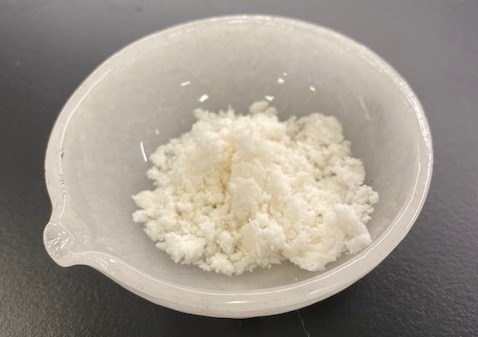
\includegraphics[width=0.7\textwidth]{produkt.jpg}}
\maketitle
\section*{Formål}
Formålet med eksperimentet er at fremstille en paraben ved en kondensationsreaktion mellem 4-hydroxybenzoesyre og ethanol.

\section*{Teori}
Parabenen i forsøget dannes ved en kondensationsreaktion mellem 4-hydroxybenzoesyre og ethanol. 
Reaktionsskemaet for denne reaktion ses i \cref{fig:kondensation}.
\begin{figure}[H]
\begin{center}
  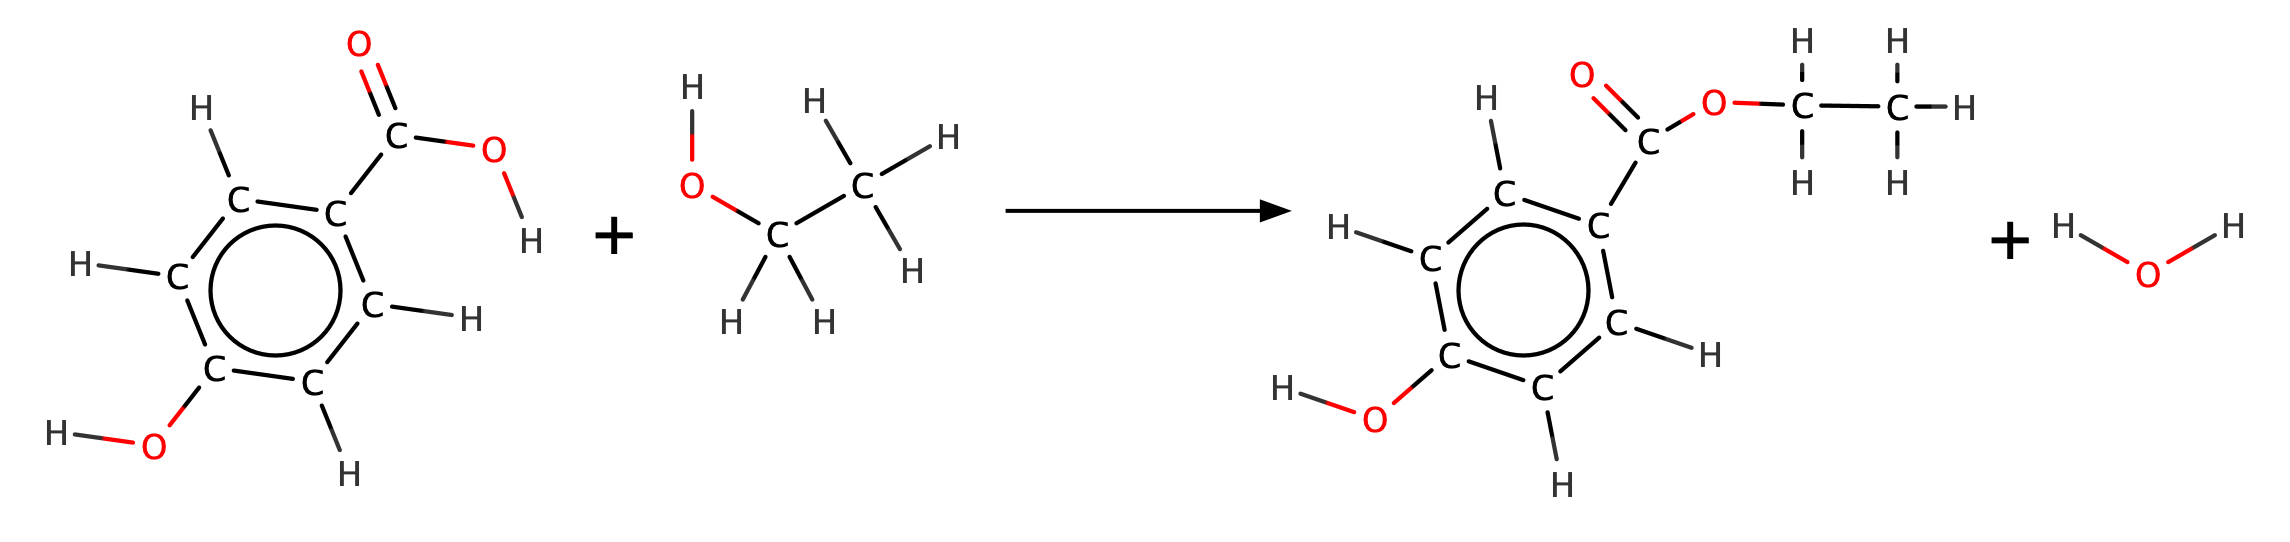
\includegraphics[width=\textwidth]{kondensation.png}
\end{center}
\caption{Reaktionsskema for reaktionen mellem 4-hydroxybenzoesyre og ethanol}
\label{fig:kondensation}
\end{figure}
\noindent Fra navngivningsreglerne for estere får vi, at parabenens systematiske navn være 4-ethyl(hydroxybenzoat).

Ved udfældningen af parabenen tilsættes en opløsning af natriumcarbonat for at fjerne den konc. svovlsyre, der har virket som katalysator.
\[
\ce{Na2CO3(aq) + H2SO4(aq) -> CO2(g) + H2O(l) + 2Na2SO4(aq)} 
\] 
Altså dannes gassen \ce{CO2} ved tilsætningen af natriumcarbonat.
\section*{Apparatur, kemikalier og sikkerhed}
\begin{multicols}{2}
\subsection*{Apparatur}
\begin{itemize}
  \item Varmeplade med magnetomrører 
\item Magnet
\item Vægt
\item Varmekappe
\item Rundbundet kolbe med slib, $250 \;\unit{mL} $
\item Korkring
\item Svaler
\item Stativ
\item Muffe og Klemme
\item Plastpipette
  \item 2 bægerglas ($250 \;\unit{mL} $) og 2 bægerglas (100 mL)
  \item 2 måleglas (50 mL)
\item Spatel
\item Udstyr til sugefiltrering
\item Porcelænsskål
\item Smeltepunktsrør og -apparat
\item Petriskål
\item Præparatglas
\end{itemize}
\end{multicols}
\subsection*{Kemikalier}
\begin{itemize}
  \item 4-hydroxybenzoesyre, \ce{HOC6H4COOH} 
  \item Methanol og ethanol
  \item Konc. svovlsyre, \ce{H2SO4} 
  \item 10 \% natriumcarbonat, \ce{Na2CO3} 
  \item Isterninger    
\end{itemize}
\subsection*{Sikkerhed}
\begin{itemize}
  \item Alkoholerne er brandfarlige og farlige ved hudkontakt, indånding og indtagelse.
  \item Konc. svovlsyre er stærkt ætsende.
  \item 4-hydroxybenzoesyre er farlig ved hudkontakt, indånding og indtagelse. 
\end{itemize}
\section*{Udførelse}
I en rundbunde kolbe afvejes omkring 5 g 4-hydroxybenzoesyre, og massen noteres ned.
Herefter overføres 30 mL ethanol til kolben, der rystes indtil 4-hydroxybenzoesyren er opløst. 
Dråbevist tilsættes så 2,5 mL konc. svovlsyre under let omrystning.
Kolben placeres så i en varmekappe med et svalerør som i \cref{fig:kog} og koges med reflux i omkring en time.
\begin{figure}[H]
\begin{center}
  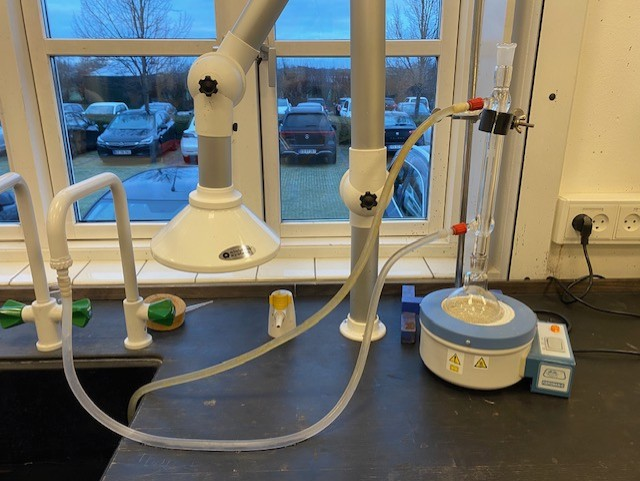
\includegraphics[width=0.7\textwidth]{kog.jpg}
\end{center}
\caption{Blandingen koges med tilbagesvaling som på billedet}
\label{fig:kog}
\end{figure}
Efter kogningen afkøles opløsning kort og overføres til et 250 mL bægerglas med 75 mL demineraliseret vand. 
Bægerglasset placeres på en magnetomrører og omrøres moderat.
Til blandingen tilsættes da 10 \% \ce{Na2CO3}, og en udfældning af parabenen sker, hvilket ses i \cref{fig:udfæld}.
Når der ikke udfældes mere af parabenen afsluttes tilsætningen af 10 \% \ce{Na2CO3}.
\begin{figure}[H]
\begin{center}
  \includegraphics[width=0.5\textwidth]{udfæld.jpg}
\end{center}
\caption{Udfældning af parabenen}
\label{fig:udfæld}
\end{figure}

Den udfældede paraben isoleres via sugefiltrering i en opstilling som i \cref{fig:sug}, og vaskes herefter tre gange igennem med isafkølet demineraliseret vand.
En smule af råproduktet gemmes til senere smeltepunktsanalyse.
\begin{figure}[H]
\begin{center}
  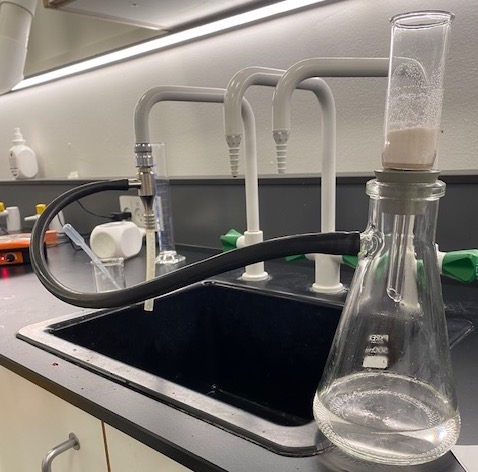
\includegraphics[width=0.5\textwidth]{sug.jpg}
\end{center}
\caption{Opstilling til sugefiltrering}
\label{fig:sug}
\end{figure}
Det frafiltrerede stof overføres til et 250 mL bægerglas, og 50 mL methanol samt 50 mL demineraliseret vand opvarmes i hver sit bægerglas under udsugning.
Derefter opløses parabenen i varm ethanol ved let omrøring.
Når parabenen er opløst tilsættes varmt vand til væsken bliver uklar.

Blandningen afkøles til stuetemperatur og de udfældede krystaller isoleres ved sugefiltrering. 
En porcelænsskål afvejes og det omkrystalliserede stof overføres til skålen (\cref{fig:prod}) og står til tørring i et par dage.
\begin{figure}[H]
\begin{center}
  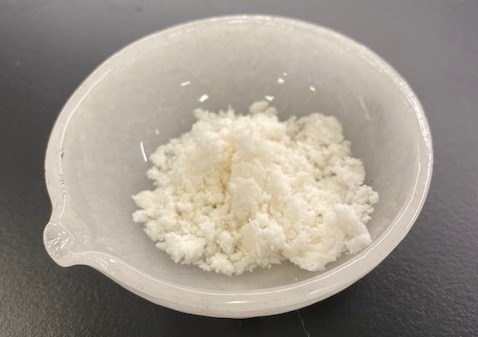
\includegraphics[width=0.7\textwidth]{produkt.jpg}
\end{center}
\caption{Det omkrystalliserede stof i porcelænsskålen}
\label{fig:prod}
Efter tørring afvejes skålen med det tørre produkt.
En smeltepunktsanalyse laves så for både råproduktet og det tørre, omkrystalliserede produkt, hvilket ses i \cref{fig:smelt}.
\begin{figure}[H]
\begin{center}
  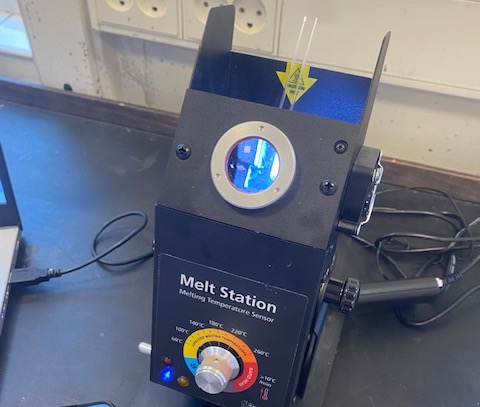
\includegraphics[width=0.7\textwidth]{smelt.jpg}
\end{center}
\caption{Smeltpunktsanalyse for råproduktet og det omkrystalliserede produkt}
\label{fig:smelt}
\end{figure}
Til sidst optages et IR-spektrum og \ce{^1H-NMR}-spektrum for det tørre, omkrystalliserede produkt.
\end{figure}

\section*{Resultater}
De noterede masser og smeltepunker ses i tabel \ref{tab:masse}.
\begin{table}[H]
  \centering
  \begin{tabular}{@{}lllll@{}}
  \toprule
    \makecell{Masse af \\porcelænsskål/g} & \makecell{Masse af porcelænsskål \\og udbytte/g} & \makecell{Målt smeltpunkt \\for råprodukt/\unit{\celsius}} & \makecell{Målt smeltepunkt for \\omkrystalliseret produkt/\unit{\celsius}}&\makecell{Masse af 4-hydroxy-\\benzoesyre/g} \\
  \midrule
    38,836 & 42,743 & 116,6-117,2 & 115,6-117,5&5,134\\
  \bottomrule
  \end{tabular}
  \caption{De noterede masser og smeltepunkter}
  \label{tab:masse}
\end{table}
Det optagede IR-spektrum for parabenen ses i \cref{fig:IR}.
\begin{figure}[H]
\begin{center}
  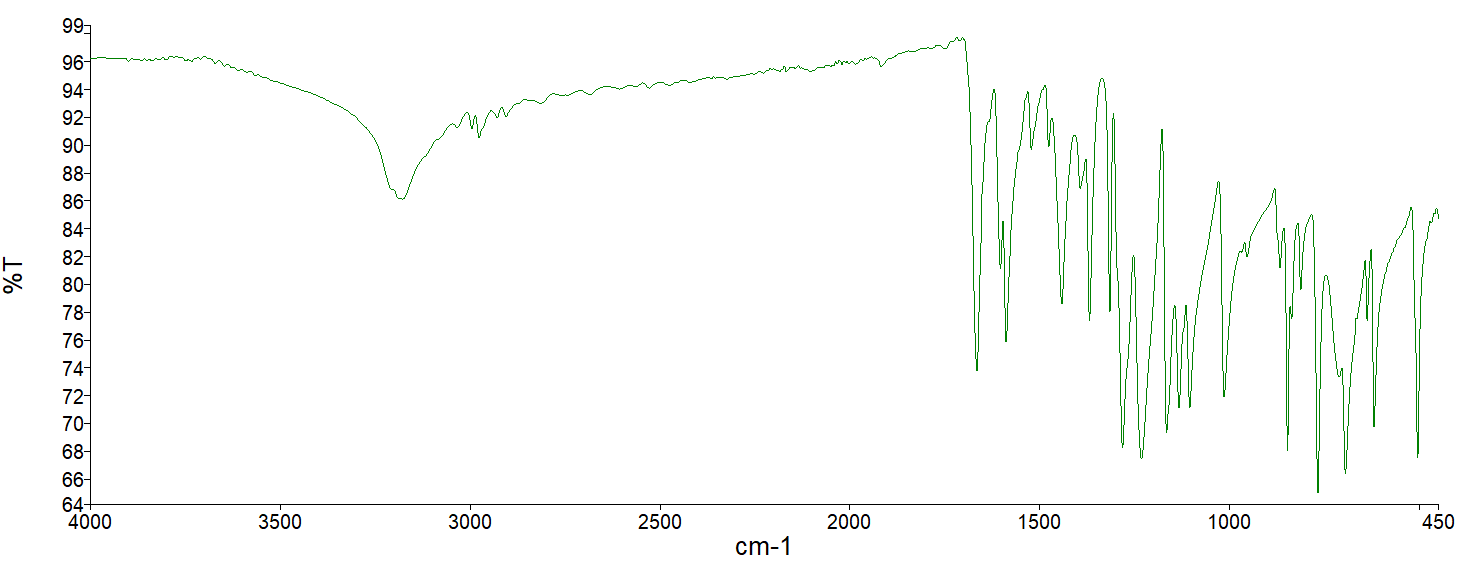
\includegraphics[width=\textwidth]{IR.png}
\end{center}
\caption{IR-spektrum for parabenen}
\label{fig:IR}
\end{figure}

\ce{^1H-NMR}-spektret for vores ethylparaben ses i \cref{fig:1HNMR}.
\begin{figure}[H]
\begin{center}
  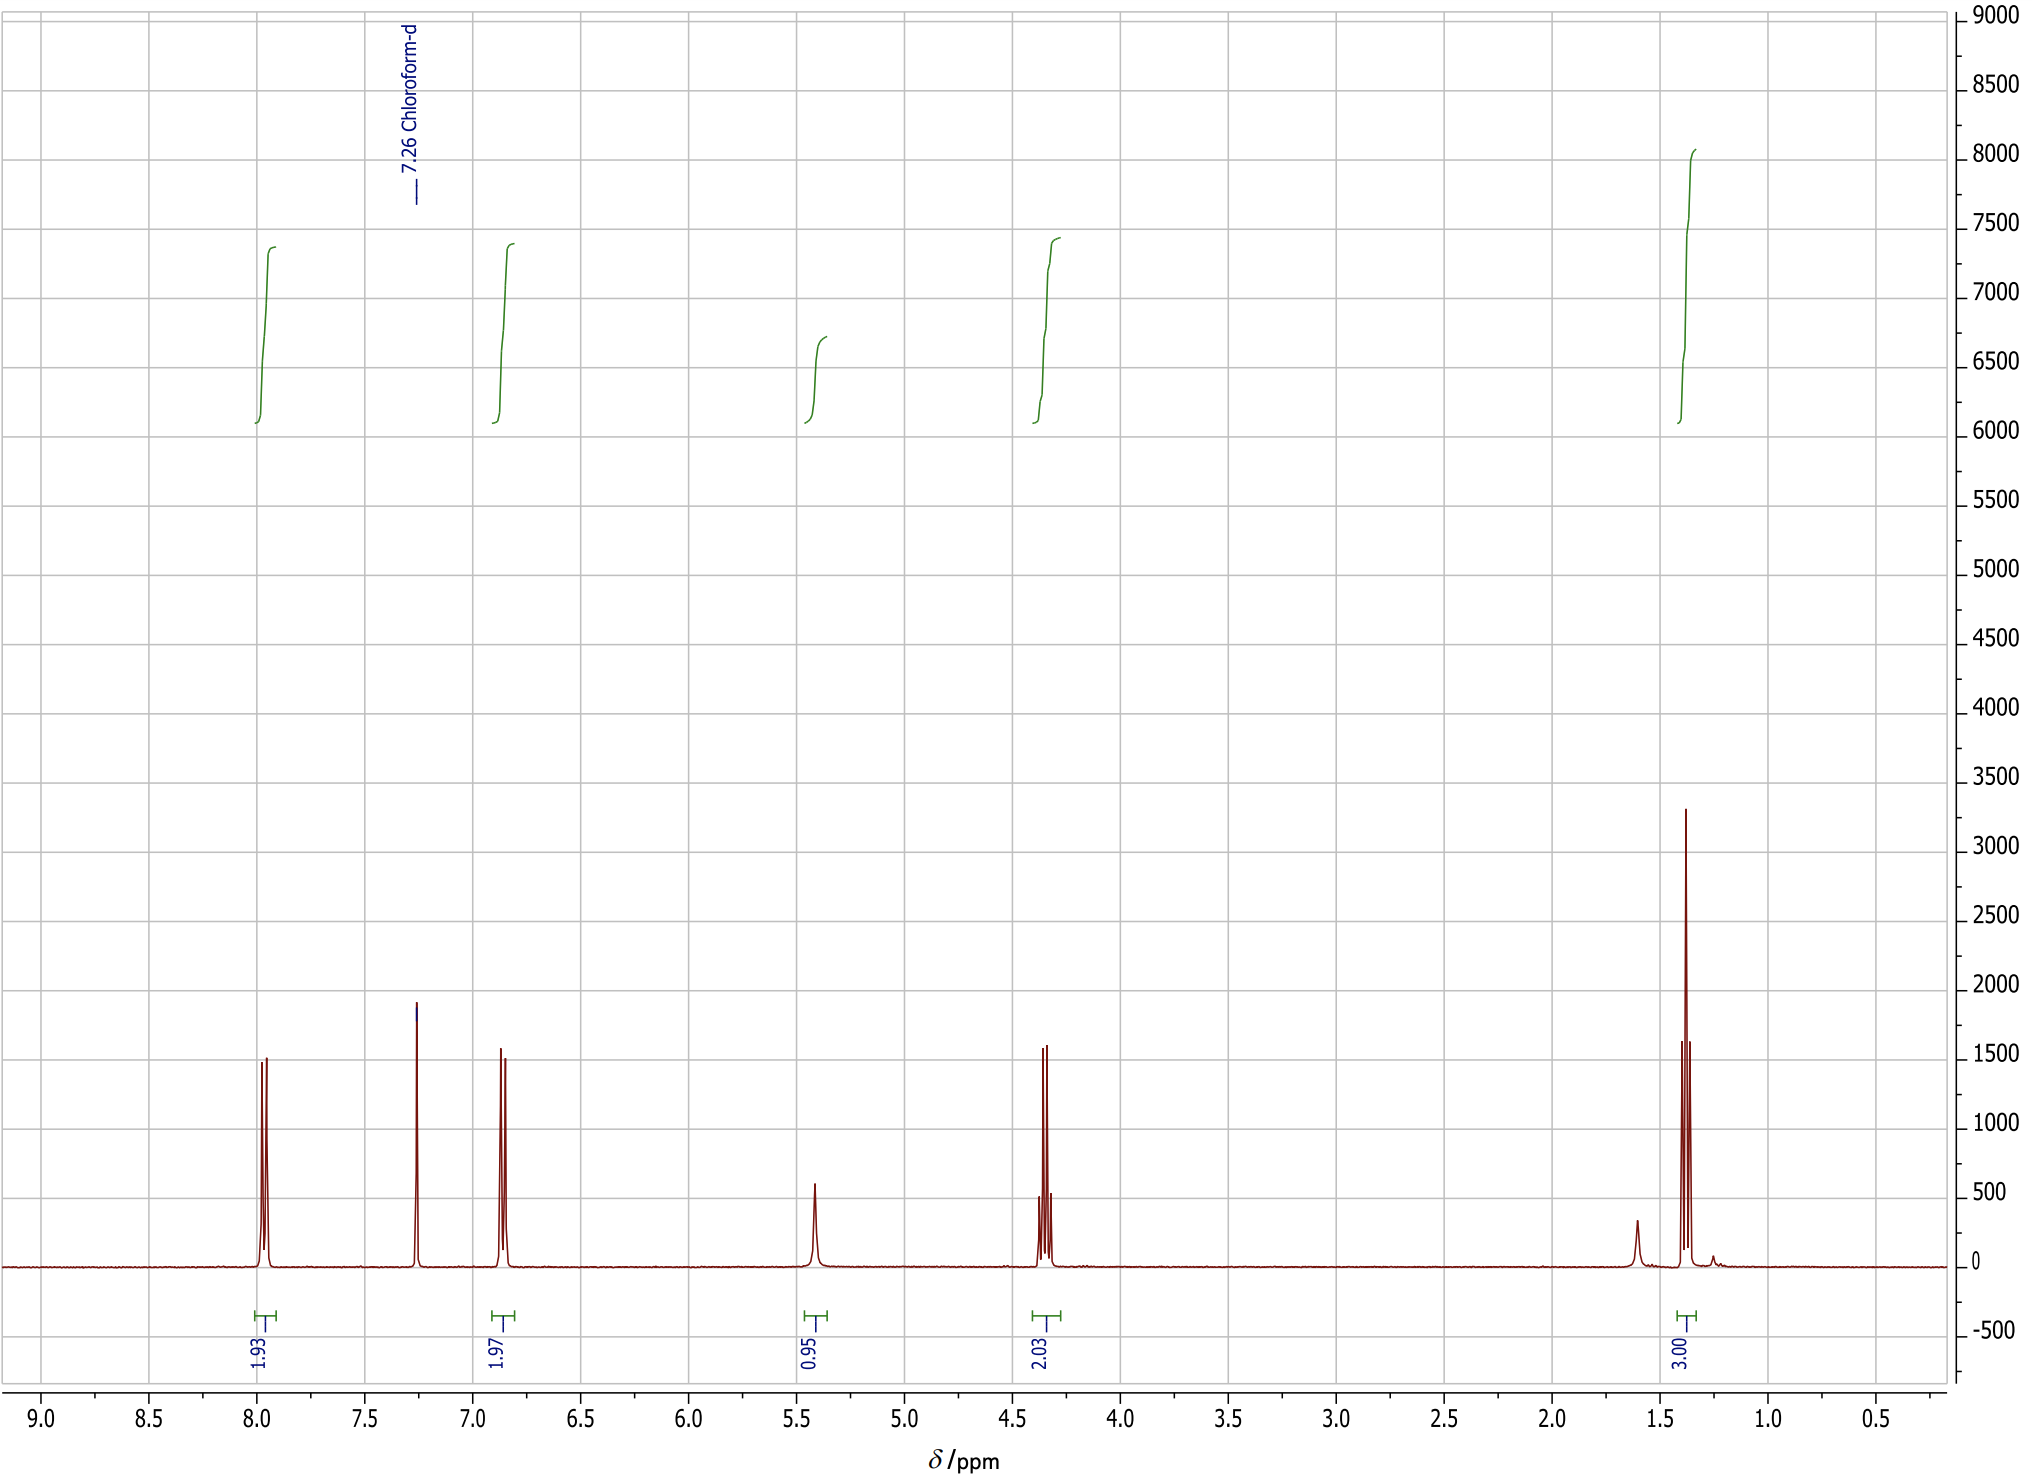
\includegraphics[width=\textwidth]{1HNMR.png}
\end{center}
\caption{\ce{^1H-NMR}-spektrum for parabenen}
\label{fig:1HNMR}
\end{figure}

\section*{Efterbehandling og sammenfatning}
Vi starter med at beregne stofmængden af den afvejede mængde 4-hydroxybenzoesyre.
\begin{equation*}
\begin{split}
  n(\text{4-hydroxybenzoesyre})&=\frac{m(\text{4-hydroxybenzoesyre})}{M(\text{4-hydroxybenzoesyre})}\\
  &=\frac{5,134 \;\unit{g} }{138,12 \;\unit{g/mol} }\\
  &=0,037170576 \;\unit{mol} \\
  &\approx 0,03717 \;\unit{mol} 
\end{split}
\end{equation*}
Vi beregner nu stofmængden af den anvendte ethanol.
\begin{equation*}
\begin{split}
  n(\text{ethanol} )&=\frac{m(\text{ethanol} )}{M(\text{ethanol} )}\\
  &=\frac{\rho(\text{ethanol} ) \cdot V(\text{ethanol} )}{M(\text{ethanol} )}\\
  &=\frac{0,789 \;\unit{g/mL} \cdot 30,0 \;\unit{mL} }{46,07 \;\unit{g/mol} }\\
  &\approx 0,514 \;\unit{mol} 
\end{split}
\end{equation*}
Vi ser da, at $n(\text{ethanol} )>n(\text{4-hydroxybenzoesyre} )$, og der er da anvendt et overskud af ethanol i reaktionen.
Det er derfor $n(\text{4-hydroxybenzoesyre})$, der bestemmer udbyttet af parabenen, og vi har
\[
n(\text{paraben} )=n(\text{4-hydroxybenzoesyre} )
\] 
og vi kan da beregne massen af det teoretiske udbytte (bemærk, at M(4-ethyl(hydroxybenzoat)) ikke findes i databogen, men kan nemt udregnes som $M(\text{ethylbenzoat}) + M(\ce{O} )$). 
\begin{equation*}
\begin{split}
  m_{\text{teo} }(\text{paraben} )&=n(\text{paraben} ) \cdot M(\text{paraben} )\\
  &=0,037170576 \;\unit{mol} \cdot 166,18 \;\unit{g/mol} \\
  &=6,17700632 \;\unit{g} \\
  &\approx 6,177 \;\unit{g} 
\end{split}
\end{equation*}
Vi beregner nu det praktiske udbytte af parabenen.
\begin{equation*}
\begin{split}
  m _{\text{prak} }(\text{paraben} )&=m(\text{porcelænsskål + udbytte} )-m(\text{porcelænsskål} )\\
  &=42,743 \;\unit{g} -38,836 \;\unit{g} \\
  &=3,907 \;\unit{g} 
\end{split}
\end{equation*}
Vi kan nu udregne det praktiske udbytte i \% af det teoretiske udbytte.
\begin{equation*}
\begin{split}
  \text{Relativt udbytte} &=\frac{m _{\text{prak} }(\text{paraben} )}{m _{\text{teo} }(\text{paraben} )}\\
  &=\frac{3,907 \;\unit{g} }{6,17700632 \;\unit{g} }\\
  &\approx 0,6325\\
  &=63,25 \% 
\end{split}
\end{equation*}
Ved opslag i Wikipedia findes, at ethylparabens smeltepunkt er $115 \;\unit{\celsius} - 118 \;\unit{\celsius} $.
Dette ligger meget tæt på de målte smeltepunkter for både råproduktet og det omkrystalliserede produkt.
En sammenfatning af de ovenstående resultater ses i \cref{tab:sam}.
\begin{table}[H]
  \centering
  \begin{tabular}{@{}lll@{}}
  \toprule
    \thead{n(4-hydroxybenzoesyre)} & \thead{n(alkohol)} & \thead{Smeltepunkt for\\ethylparaben (tabel)} \\
  \midrule
    0,03717 mol & 0,5139 mol & $115 \;\unit{\celsius} - 118 \;\unit{\celsius} $\\
  \toprule
    \thead{Teoretisk udbytte\\ m(paraben)}&\thead{Praktisk udbytte\\m(paraben)} &\thead{Udbytte i \%} \\
  \midrule
    6,177 g & 3,907 g &63,25\%\\
  \bottomrule
  \end{tabular}
  \caption{Sammenfatning af efterbehandling}
  \label{tab:sam}
\end{table}
En tilordning af de karakteristiske absorptionsbånd over $1500 \;\unit{cm^{-1}} $ i IR-spektret ses i \cref{tab:IR}.
\begin{table}[H]
  \centering
  \begin{tabular}{@{}llllll@{}}
  \toprule
    \makecell{Bånd\\nr.} & \makecell{$\frac{1}{\lambda }$/\unit{cm^{-1}}\\(aflæst)} & Intensitet & Bindingstilordning & Kommentarer & \makecell{$\frac{1}{\lambda }$/\unit{cm^{-1}}\\(tabel)}\\
  \midrule
   1 & 3200-3000 & Svag-medium & \ce{O-H} strækning & \makecell{Alkohol/phenol\\Bredt bånd} & 3100-3600 \\
    2 & 2900-3000 & Svage & \makecell{\ce{ C-H} strækning\\C:$sp^3$} & \makecell{Alkyl\\Flere bånd} & 2810-2960 \\
    3 & 1750 & Medium & \ce{ C=O} strækning & Ester & 1745 \\
    4 & 1600 & Medium & \makecell{ \ce{C\bond{~-}C} strækning\\C:$sp^2$}&\makecell{Aromatisk ring\\To bånd} & 1575-1600 \\
  \bottomrule
  \end{tabular}
  \caption{Tilordning af absorptionsbånd i IR-spektret}
  \label{tab:IR}
\end{table}
Vi ser da, at det i høj grad er i overensstemmelse med strukturformlen for parabenen, der ses i \cref{fig:kondensation}.
Der mangler dog et bånd for \ce{C-H}-strækningsvibrationer, hvor \ce{C}-atomet er $sp^2$-hybridiseret (bølgetal på 3010-$3100 \;\unit{cm^{-1}} $).
Dette kan være forårsaget af, at den bliver "slugt" af bånd nr. 1.

En tilordning af signalerne i \ce{^1H}-NMR-spektret af parabenen ses i \cref{tab:HNMR}.
\begin{table}[H]
\centering
\begin{tabular}{@{}lllllll@{}}
\toprule
  \makecell{Signal\\nr.} & \makecell{Kemisk skift\\(aflæst)\\$\delta$/ppm}& \makecell{Integral/areal\\(relativt antal ækvi-\\valente \ce{^1H}-atomer)}  & Opsplitning & Antal nabo-\ce{^1H}'er  & Tilordning & \makecell{Kemisk skift\\(tabel)\\$\delta$/ppm} \\
\midrule
  1 & 1,4 & 3 & Triplet & 2 & \ce{C\textbf{H}3-CH2-CO-O} & 1,2 \\
  2 & 4,3 & 2 & Kvartet & 3 & \ce{CH3-C\textbf{H}2-O-CO-Ar} & 4,4 \\ 
  3 & 5,4 & 1 & Singlet & 0 & \ce{Ar-OH} & 4,5-10\\
  4 & 6,85 & 2 & Dublet & 1 & \ce{2 Ar-H} & 6,5-8\\
  5 & 7,95 & 2 & Dublet & 1 & \ce{2 Ar-H} & 6,5-8 \\
\bottomrule
\end{tabular}
\caption{Tilordning af absorptionsbånd i \ce{^1H}-NMR-spektret}
\label{tab:HNMR}
\end{table}
\noindent De \ce{^1H}-atomer, som signalerne svarer til ses i \cref{fig:signal}.
\begin{figure}[H]
\begin{center}
  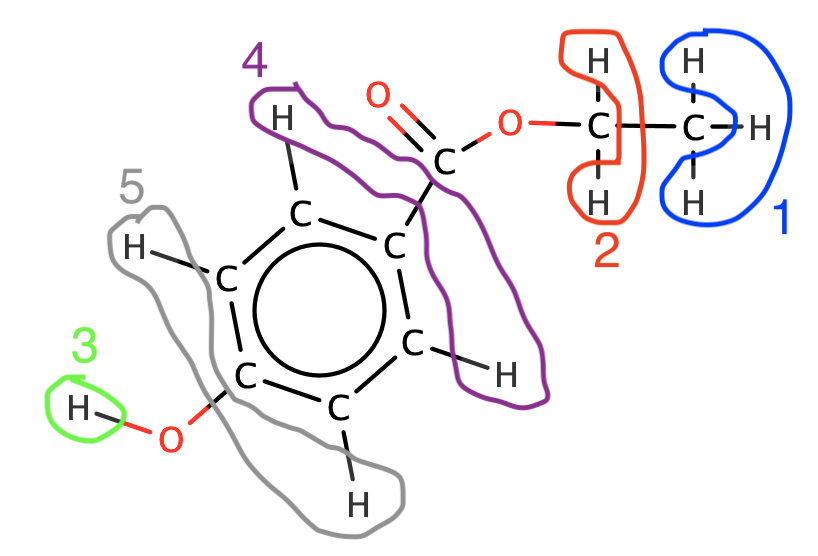
\includegraphics[width=\textwidth]{signal.png}
\end{center}
\caption{De tilsvarende \ce{^1H}-atomer til signalerne}
\label{fig:signal}
\end{figure}
\ce{^1H}-NMR-spektret passer altså med strukturformlen for ethylparaben, og det fremstillede stof må da være det ønskede paraben.

\section*{Mulige fejlkilder}
Den største årsag til, at udbyttet ikke er højere, er besvær med at få alt produktet ud af sugefilteret.
Derudover benyttes noget af råproduktet til smeltepunktsanalyse.

\section*{Konklusion}
Vi har fremstillet ethylparaben ved en kondensationsreaktion mellem 4-hydroxybenzoesyre og ethanol.
Dette er gjort med et relativt udbytte på $63,25 \%$.

\end{document}
